\documentclass[conference]{IEEEtran}

\usepackage{cite}
\usepackage{amsmath,amssymb}
\usepackage{graphicx}
\usepackage{xcolor}
\usepackage{url}
\usepackage{tikz}
\usetikzlibrary{arrows.meta,positioning,shapes.geometric}

\setlength{\headheight}{26pt}

\makeatletter
\def\ps@IEEEtitlepagestyle{%
  \def\@oddhead{%
    \parbox{\textwidth}{\centering\footnotesize
    \textbf{CSE 440 -- Artificial Intelligence; Section: 1} \hspace{1em}
    \textbf{Project Group: 8}\\
    Nafiz Un Nabi Ishan (2121346042); Abdullah Al Towhid (2031045042);\\
    Ruddro Debnath Badhon (2021009642); Saif Mahmood Chowdhury (2132325642)}}
  \def\@evenhead{\@oddhead}
  \def\@oddfoot{\hfill\thepage\hfill}
  \def\@evenfoot{\@oddfoot}
}
\makeatother

\title{Project Update Report: Midpoint Progress on \texttt{Mystery\_Solver}, a Bayesian Network-Based Interactive Mystery Solver}

\author{\IEEEauthorblockN{Group 8}}

\begin{document}

\maketitle
\thispagestyle{IEEEtitlepagestyle}
\pagestyle{plain}

\begin{abstract}
This report covers the midpoint progress of \texttt{Mystery\_Solver}, a course project that demonstrates probabilistic reasoning through a Bayesian Network-based mystery-solving application. The system estimates the most likely culprit in a fictional manuscript theft by combining prior suspect probabilities with user-supplied clues---forced entry, alibis, fingerprints, and security footage. So far, the core problem has been formulated, the software stack finalized, the Bayesian model built, and a working interactive prototype delivered. The backend runs on Python and \texttt{pgmpy}; the frontend uses Streamlit. The remaining work covers environment reproducibility, interface integration, CPD documentation, and testing.
\end{abstract}

\begin{IEEEkeywords}
Bayesian network, project update, probabilistic inference, Streamlit, pgmpy, educational AI application
\end{IEEEkeywords}

\section{Introduction}
Reasoning under uncertainty is a core problem in artificial intelligence. Most real-world systems must make decisions from incomplete or ambiguous information, and Bayesian Networks are a well-established way to handle this---they encode dependencies between variables as a directed probabilistic graph and support posterior inference from observed evidence \cite{pearl1988}. The formalism is mathematically grounded and, crucially, still readable enough to trace what the model is actually doing, which makes it a good fit for an educational project.

\texttt{Mystery\_Solver} is an interactive application that puts this reasoning in front of a user through a fictional scenario. The user enters clues, and the model updates the probability that each suspect is guilty. The aim is a working browser-based tool that demonstrates the core ideas clearly---not a research system. This report describes where the project stands at the halfway point.

\section{Project Objective and Current Scope}
The scenario involves a stolen manuscript and three suspects: the Scholar, the Butler, and the Cat Burglar. Given clues from the user, the system computes a posterior distribution over these suspects, illustrating how prior belief and observed evidence interact in Bayesian inference \cite{zhang1996}.

The current version uses a single hidden cause variable, \texttt{GuiltyParty}, with observable evidence nodes for forced entry, suspect-specific alibis, fingerprints, and security footage. The scope was kept narrow on purpose---getting the inference correct was the priority before expanding the variable set. The second half of the project shifts focus to reproducibility, cleaner documentation, and making the tool presentable as an academic artifact.

\section{Methodology and Preliminary Model Design}
The project uses a discrete Bayesian Network implemented in \texttt{pgmpy} \cite{ankpan2015,pgmpydocs}. \texttt{GuiltyParty} is the parent of every evidence node, so the model assumes clue variables are conditionally independent given the true culprit. The joint distribution is:
\begin{equation}
P(G,E_1,\ldots,E_m)=P(G)\prod_{i=1}^{m}P(E_i \mid G),
\end{equation}
where \(G\) denotes the guilty party and \(E_i\) denotes each observed clue.

The prior is currently uniform across the three suspects:
\begin{equation}
P(G=A)=P(G=B)=P(G=C)=\frac{1}{3}.
\end{equation}
Conditional probability distributions (CPDs) were assigned manually based on narrative logic. Forced entry is modeled as far more likely if the Cat Burglar is guilty; a missing alibi raises the posterior for the corresponding suspect. Inference uses variable elimination, available directly in \texttt{pgmpy} \cite{pgmpydocs}. These CPD assignments will be explained more systematically in the final report.

The network structure is shown in Fig.~\ref{fig:update_bn}.

\begin{figure}[!h]
\centering
\resizebox{0.9\columnwidth}{!}{%
\begin{tikzpicture}[
  node distance=0.9cm and 0.95cm,
  var/.style={draw, circle, align=center, minimum size=1cm},
  arrow/.style={-{Latex[length=2mm]}, thick}
]
\node[var] (g)  {\texttt{G}};
\node[var, above left=of g]  (fe) {\texttt{FE}};
\node[var, above=of g]       (aa) {\texttt{A\_A}};
\node[var, above right=of g] (ab) {\texttt{A\_B}};
\node[var, below left=of g]  (ac) {\texttt{A\_C}};
\node[var, below=of g]       (fp) {\texttt{FP}};
\node[var, below right=of g] (sf) {\texttt{SF}};
\draw[arrow] (g) -- (fe);
\draw[arrow] (g) -- (aa);
\draw[arrow] (g) -- (ab);
\draw[arrow] (g) -- (ac);
\draw[arrow] (g) -- (fp);
\draw[arrow] (g) -- (sf);
\end{tikzpicture}}
\caption{Bayesian Network structure used in the current prototype. \texttt{G} = GuiltyParty; \texttt{FE} = ForcedEntry; \texttt{A\_A}, \texttt{A\_B}, \texttt{A\_C} = suspect alibis; \texttt{FP} = Fingerprints; \texttt{SF} = SecurityFootage.}
\label{fig:update_bn}
\end{figure}

\section{Implementation Progress to Date}
The software stack is chosen and partially implemented. Python is the project language \cite{pythondocs}. \texttt{pgmpy} handles the probabilistic model and Streamlit provides the browser interface \cite{streamlitdocs}. Graphviz has been considered for rendering the network structure visually \cite{graphvizdocs}.

A working prototype exists. The application collects evidence through sidebar controls, assembles an evidence dictionary, runs posterior inference, and displays the resulting probability distribution over suspects. The main AI mechanism is therefore already functional, though the artifact is still an early prototype rather than a finished system.

\section{Current Issues and Remaining Work}
Several tasks remain before the final submission. The virtual environment is currently machine-specific, so a clean, reproducible setup process needs to be defined. Motive-related interface controls exist in the sidebar but are not yet wired into inference. The CPD values are heuristic and need clearer justification in writing. Automated tests and documentation are also incomplete.

The harder part of the project---taking an idea and turning it into a working Bayesian inference system---is done. What remains is refinement and polish.

\section{Conclusion}
\texttt{Mystery\_Solver} has reached a solid midpoint. The graph structure is defined, CPDs are specified, exact inference runs correctly through \texttt{pgmpy}, and a Streamlit interface is in place. The remaining work is well-scoped: reproducibility, interface integration, documentation, and testing. The project is on track for a complete final submission.

\section*{Acknowledgment}
This report was prepared from direct inspection of the project code and files. ChatGPT by OpenAI was used as a writing assistance tool for organizing and refining the report text; all project-specific technical statements were verified against the implementation and official documentation \cite{chatgpt}.

\begin{thebibliography}{99}

\bibitem{pearl1988}
J. Pearl, \textit{Probabilistic Reasoning in Intelligent Systems: Networks of Plausible Inference}. San Mateo, CA, USA: Morgan Kaufmann, 1988.

\bibitem{zhang1996}
N. L. Zhang and D. Poole, ``Exploiting causal independence in Bayesian network inference,'' \textit{Journal of Artificial Intelligence Research}, vol. 5, pp. 301--328, 1996, doi: 10.1613/jair.305.

\bibitem{ankpan2015}
A. Ankan and A. Panda, ``pgmpy: Probabilistic Graphical Models using Python,'' in \textit{Proceedings of the 14th Python in Science Conference}, 2015, pp. 6--11, doi: 10.25080/Majora-7b98e3ed-001.

\bibitem{pgmpydocs}
``pgmpy Documentation,'' pgmpy. [Online]. Available: \url{https://pgmpy.org/}. Accessed: Apr.~27, 2026.

\bibitem{streamlitdocs}
``Streamlit Documentation,'' Streamlit. [Online]. Available: \url{https://docs.streamlit.io/}. Accessed: Apr.~27, 2026.

\bibitem{graphvizdocs}
``Graphviz Documentation,'' Graphviz. [Online]. Available: \url{https://graphviz.org/documentation/}. Accessed: Apr.~27, 2026.

\bibitem{pythondocs}
``Python Documentation,'' Python Software Foundation. [Online]. Available: \url{https://docs.python.org/}. Accessed: Apr.~27, 2026.

\bibitem{chatgpt}
``ChatGPT Overview,'' OpenAI. [Online]. Available: \url{https://openai.com/chatgpt/overview/}. Accessed: Apr.~27, 2026.

\end{thebibliography}

\end{document}